\documentclass[a4paper, 12pt]{article}

% čeština
\usepackage[utf8]{inputenc}

\usepackage{ifxetex}
\ifxetex
  \usepackage{fontspec}
  \usepackage{xltxtra}
  \usepackage[czech]{babel}
\else
  \usepackage[cp1250]{inputenc}
  \usepackage[czech]{babel}
\fi
%%

\usepackage{bakalarska_prace}
\usepackage{url}

%% kód
\usepackage{listings}
 
\definecolor{codegreen}{rgb}{0,0.6,0}
\definecolor{codegray}{rgb}{0.5,0.5,0.5}
\definecolor{codedarkcyan}{rgb}{0,0.55,0.55}
\definecolor{backcolour}{rgb}{0.985,0.985,0.985}
\definecolor{keywordblue}{rgb}{0.15,0.29,0.55}
 
\lstdefinestyle{mystyle}{
    backgroundcolor=\color{backcolour},   
    commentstyle=\color{codegreen},
    keywordstyle=\color{keywordblue},
    numberstyle=\tiny\color{codegray},
    stringstyle=\color{codedarkcyan}\ttfamily,
    basicstyle=\ttfamily\footnotesize\lgweight,
    breakatwhitespace=false,         
    breaklines=true,                 
    captionpos=b,                    
    keepspaces=true,                 
    numbers=left,                    
    numbersep=5pt,                  
    showspaces=false,                
    showstringspaces=false,
    showtabs=false,                  
    tabsize=2
}
\lstset{style=mystyle}
%%

% grafika
\usepackage{graphicx}
\usepackage{caption}
\usepackage{color, soul}
\usepackage{xcolor}
\usepackage[most]{tcolorbox}
\newtcolorbox{highlighted}{colback=yellow!40,coltext=black,breakable}
% okraje (v případě potřeby):\usepackage[showframe]{geometry}
%%

% poznámky
\usepackage[colorinlistoftodos]{todonotes}
\newcommand\todoin[2][]{\todo[inline, caption={2do},#1]{\begin{minipage}{\textwidth-4pt}#2\end{minipage}}}
\definecolor{lavender}{rgb}{0.96, 0.73, 1.0}

%%


\begin{document}


% souhrn
% (CZ)
\section*{Souhrn}
Při reaktivní sintraci dochází působením tlaku a tepla ke spékání práškových kovů za vzniku jejich sloučenin. Pro zkoumání mechanismu a kinetiky tohoto děje se využívá snímání reakční směsi pomocí rentgenové difrakce $in$ $situ$. Z takto získaných dat lze zpětně vizuálním posouzením přibližně identifikovat  moment vzniku jednotlivých intermetalických sloučenin. Cílem této práce bylo vytvořit program s uživatelským rozhraním umožňující efektivnější analýzu krystalografických dat s důrazem na přesnost identifikace vznikajících fází. Vzniklý program je vybaven nástroji pro načítání dat ze souborů, jejich vizualizaci a zpracování signálu. Program rovněž umožňuje zpracovaná data zpětně exportovat do souborů. K tvorbě programu byl využit programovací jazyk Python.

% (EN)
\section*{Summary}
During the reactive sintering, powdery metals are sintered at high temperatures and under pressure to form their compounds. To study the mechanism and kinetics of this process, the X-ray diffraction real-time capturing of the reaction mixture is used. From the obtained data, the moment of appearance of each intermetallic compound can be identified. The aim of this work was to create a program with user interface enabling more efficient analysis of crystallographic data with an emphasis on the accuracy of identification of emerging phases. The program is equipped with tools for data retrieval, visualization and signal processing. The program also allows the user to export processed data back to files. The program was created within the Python programming language.
%%
\newpage

% poděkování
\section*{Poděkování}
případné poděkování. Pokud není, stranu vynechat.
%%
\newpage

% obsah
\tableofcontents
%%
\newpage

% úvod
\section{Úvod}
Úvod.
%%

% teoretická část
\section{Python}
V této kapitole bude představen programovací jazyk Python (\ref{sec:history})
\subsection{Stručná historie Pythonu} \label{sec:history}
V 80. letech minulého století pracovali vývojáři institutu Centrum voor Wiskunde en Informatica (CWI) v Nizozemsku na skriptovacím jazyku ABC.  Ten měl být určen uživatelům z řad veřejnosti bez širších programátorských znalostí. \cite{PythonHist:1} Přes snahu jeho tvůrců se toho ale nepodařilo dosáhnout. Z toho důvodu se Guido van Rossum rozhodl vytvořit nový, uživatelsky přívětivější jazyk, který by odstranil nedostatky jazyka ABC. První verze tohoto jazyka nazvaného Python byla vypuštěna v roce 1994. \cite{PythonHist:2}
\\
\noindent
Od té doby prošel Python značným vývojem a dočkal se mnoha nových verzí, z nichž zatím poslední (verze 3.7.3) byla zveřejněna k 25. březnu letošního roku (2019). \cite{PythonVersion}

\subsection{Specifika programování v Pythonu} \label{sec:specifika}
Python je multimodální skriptovací jazyk umožňující programování v rámci jak objektově orientovaného, tak procedurálního paradigmatu. \cite{Python3Summerfield:1} \todoin[bordercolor=green!80, backgroundcolor=green!30]{Kam umístit citaci, když více částí odstavce pochází ze stejného zdroje?}
\todo[bordercolor=lavender,backgroundcolor=lavender!40,linecolor=lavender]{statistika/\\graf}
\noindent Jedná se o velmi oblíbený programovací jazyk hned z několika z důvodů. Hlavním z nich je srozumitelnost produkovaného kódu a tudíž jeho snadná osvojitelnost i pro uživatele bez větších zkušeností s programováním. S tím souvisí široká uživatelská komunita, která je, vedle propracované dokumentace, důležitým nástrojem při řešení problémů.  Jedná se rovněž o multiplatformní jazyk, tj. programy v něm napsané lze bez větších problémů spustit prakticky v libovolném systému, ať už Windows nebo v systémech na bázi Unix (Linux, Mac OS X apod.). V neposlední řadě je značnou výhodou Pythonu jeho rozsáhlá standardní knihovna, která umožňuje celou řadu úkonů. Zároveň je ale pro specializované operace k dispozici velké množství doplňkových knihoven třetích stran.
\\
\\
\noindent
Jak již bylo řečeno, Python je především objektově orientovaným jazykem. Podstatu objektově orientovaného přístupu tvoří tzv. objekty. Objekty jsou seskupení dat s určitými vlastnostmi a funkcionalitami pracující na principu černé skříňky, tj. vykonávají určité činnosti a komunikaci s okolím bez nutnosti znát jejich vnitřní podstatu. Nadřazeným prvkem objektu je datový typ, neboli třída. Ten sdružuje samotné objekty a také operace, které je možné s nimi provádět. Příkladem může být např. třída \texttt{int} a do ní náležící objekt, číslo \texttt{3}. Třída \texttt{int} tedy zaštiťuje celá čísla s přesností na několik desetinných míst (angl.\textit{ integers}), s nimiž je možné provádět matematické operace, seskupovat je do seznamů, apod. \todoin[bordercolor=lavender, backgroundcolor=lavender!40]{Pro mě: ještě jeden příklad, příp. celkově lepší formulace poslední věty.}

\\
\noindent
Výhoda použití objektově-orientovaného přístupu spočívá v tzv. dědičnosti, díky níž objekty náležící do určité podtřídy odvozené od třídy hlavní přebírají (dědí) její vlastnosti. Tím dochází k úspoře vyprodukovaného kódu, neboť tyto objekty z podtříd není nutné znovu specifikovat. Vzniklý kód je tak přehlednější a celkově úspornější. Toho lze využít např. při tvorbě uživatelských rozhraní, kdy jsou kladeny nároky především na velikost skriptu. \ldots

\subsection{Grafické uživatelské rozhraní} \label{sec:GUI}
Grafické uživatelské rozhraní, zkráceně GUI (z angl. \textit{Graphical User Interface}), je nástroj, s jehož pomocí je realizována oboustranná interakce mezi programem a uživatelem. Směrem dovnitř přicházejí vstupy zadané uživatelem, na než následně reagují odpovídající výstupy programu. Vstupy jsou uživatelem vysílány pomocí interaktivních ovládacích prvků, tzv. \textcolor{lavender}{widgetů}, např. ve formě tlačítek, posuvníků, rolovacích seznamů apod. Výstupy programu se pak mohou projevovat rovněž nejrůznější způsoby, ať už jako procesy na pozadí nebo přímo akcemi v rámci grafických oken programu. Vnitřní podstatu fungování GUI si pak lze představit jako jakousi \uv{nekonečnou} smyčku událostí, která je vyvolána spuštěním programu a vytvořením hlavního okna s jeho ovládacími prvky. Ta následně čeká na vstup zvenčí. Pakliže takový vstup nepřichází, setrvává ve vyčkávací pozici. Jakmile jej ale dostane, postupuje dle předepsaného algoritmu až na konec, poté se opět vrátí do vyčkávací pozice. Tento cyklus se opakuje do té doby, než uživatel vyšle signál k ukončení programu. Tento proces je schematicky znázorněn na obr. č. \ref{fig:Gui} (převzato z \cite{Python3Summerfield:2} a upraveno).
\begin{figure}[hbt!]
    \centering
    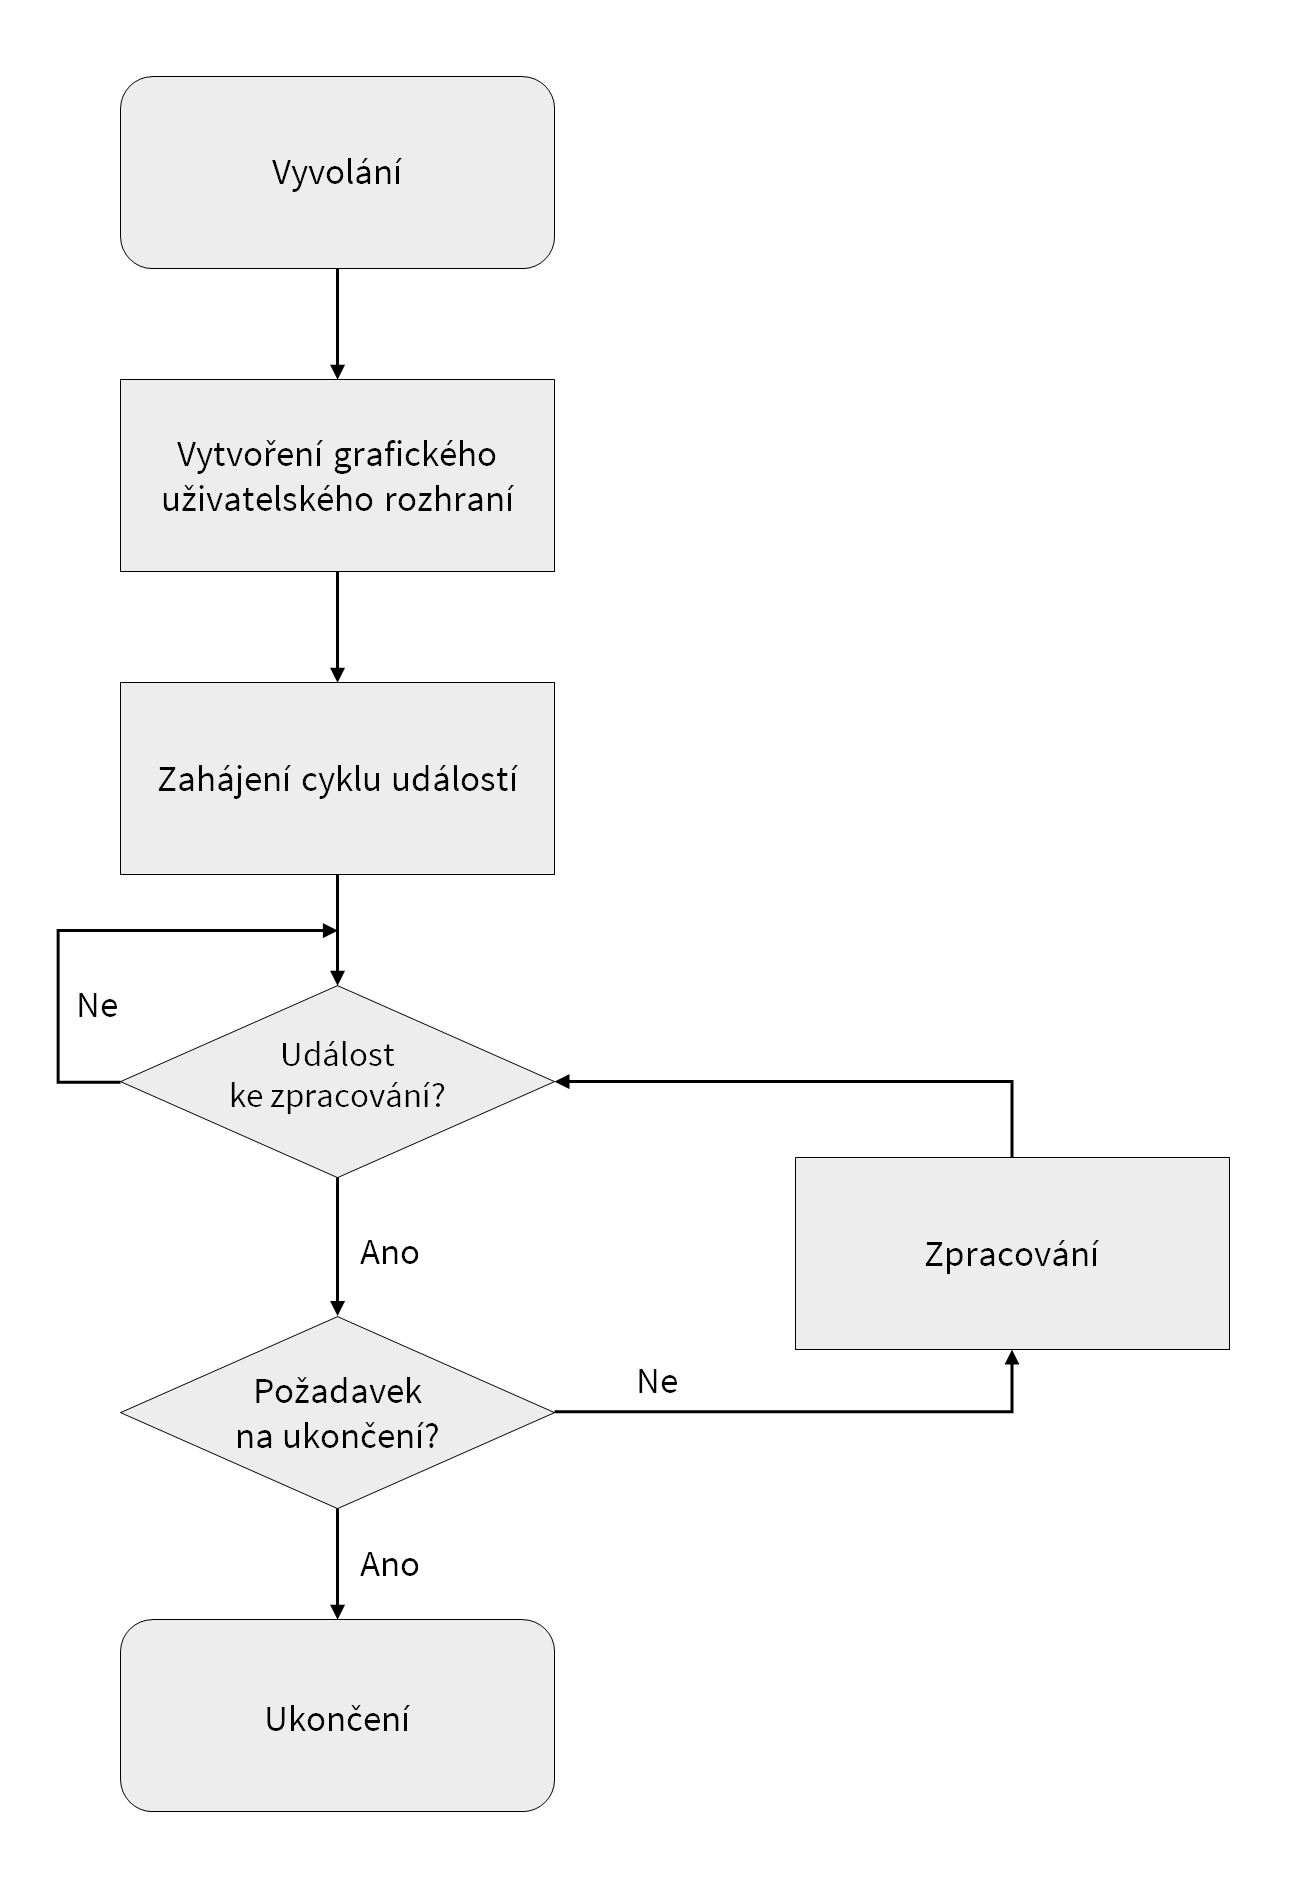
\includegraphics{gui_princip.png}
    \caption{Princip fungování programu vybaveného grafickým uživatelským rozhraním}
    \label{fig:Gui}
\end{figure}

\subsubsection{Tvorba GUI v Pythonu}
 Realizaci grafického uživatelského rozhraní lze v Pythonu provést hned několika způsoby. K dispozici je celá řada tzv. frameworků, tedy souborů specializovaných balíčků a modulů pro tvorbu GUI. Tato práce se však zaměřuje pouze na dva z nich, a to na PyQt a tkinter, za účelem jejich porovnání. PyQt je framework, v němž byl vytvořen program, jenž je předmětem této práce. tkinter byl zvolen k porovnání z důvodu, že se jedná o obecně nejčastěji používaný modul pro tvorbu uživatelských rozhraní v jazyce Python.
\subsubsection*{tkinter}
Obliba tkinter pramení pravděpodobně z toho, že se jedná o vestavěný modul Pythonu, tj. je součástí jeho standardní instalace spolu s knihovnou GUI Tk. To představuje značnou výhodu zejména v případě, že uživatel má k dispozici pouze standardní instalaci Pythonu a nechce či nemůže instalovat knihovny třetích stran. \cite{Python3Summerfield:2} Zároveň je tkinter frameworkem s poměrně malými nároky na paměť a jednoduchou syntaxí. Je tak vhodný zejména pro začátečníky. S tím se ale také pojí jeho hlavní nevýhoda, kterou je omezená nabídka widgetů, kvůli níž programy v něm vyprodukované působí méně nativně. tkinter tak není sám o sobě vhodný k tvorbě složitějších aplikací a je proto žádoucí jej, pokud možno, kombinovat s dalšími knihovnami. Co se týče kvality kódu, tkinter ve srovnání s knihovnami třetích stran opět kulhá. Obecně programy používající k tvorbě GUI jiné knihovny než Tk poskytují při stejné nebo kratší délce kódu výrazně lepší výsledky. \cite{Python3Summerfield:2}  

\subsubsection*{PyQt}
PyQt je odnoží od multiplatformního frameworku Qt určenou speciálně pro Python. Qt je samo o sobě knihovnou jazyka C++, ale podobně jako pro Python existuje v mnoha modifikacích i pro mnoho dalších skriptovacích jazyků (Ruby - \texttt{QtRuby}, C\texttt{\#}, Pascal, Java, atd.). Výhodou Qt je přehledná a podrobná dokumentace (společná pro všechny odnože), snadná instalace, kterou je možné provádět přes příkaz \texttt{pip} v příkazovém řádku a také nízké nároky na paměť. Aplikace vytvořené v Qt, resp. PyQt jsou také nativní, tj. přizpůsobují svůj vzhled operačnímu systému, na kterém jsou spuštěny. PyQt rovněž nabízí možnost využití nástroje QtDesigner, což je vývojové prostředí umožňující \textcolor{lavender}{klikáním} poskládat grafické rozhraní z nabídky jednotlivých ovládacích prvků (viz obr. \ref{fig:QtDesigner}). Z prostředí QtDesigneru je dále možné generovat kód vytvořeného GUI do Pythonu a do něj ručně vepsat funkcionality jednotlivých widgetů. Nevýhodou použití tohoto nástroje je ale množství a značná nepřehlednost generovaného kódu, neboť se v něm promítají veškeré programátorem \uv{\textcolor{lavender}{naklikané}} změny.
\newline
\begin{figure}[hbt!]
    \centering
    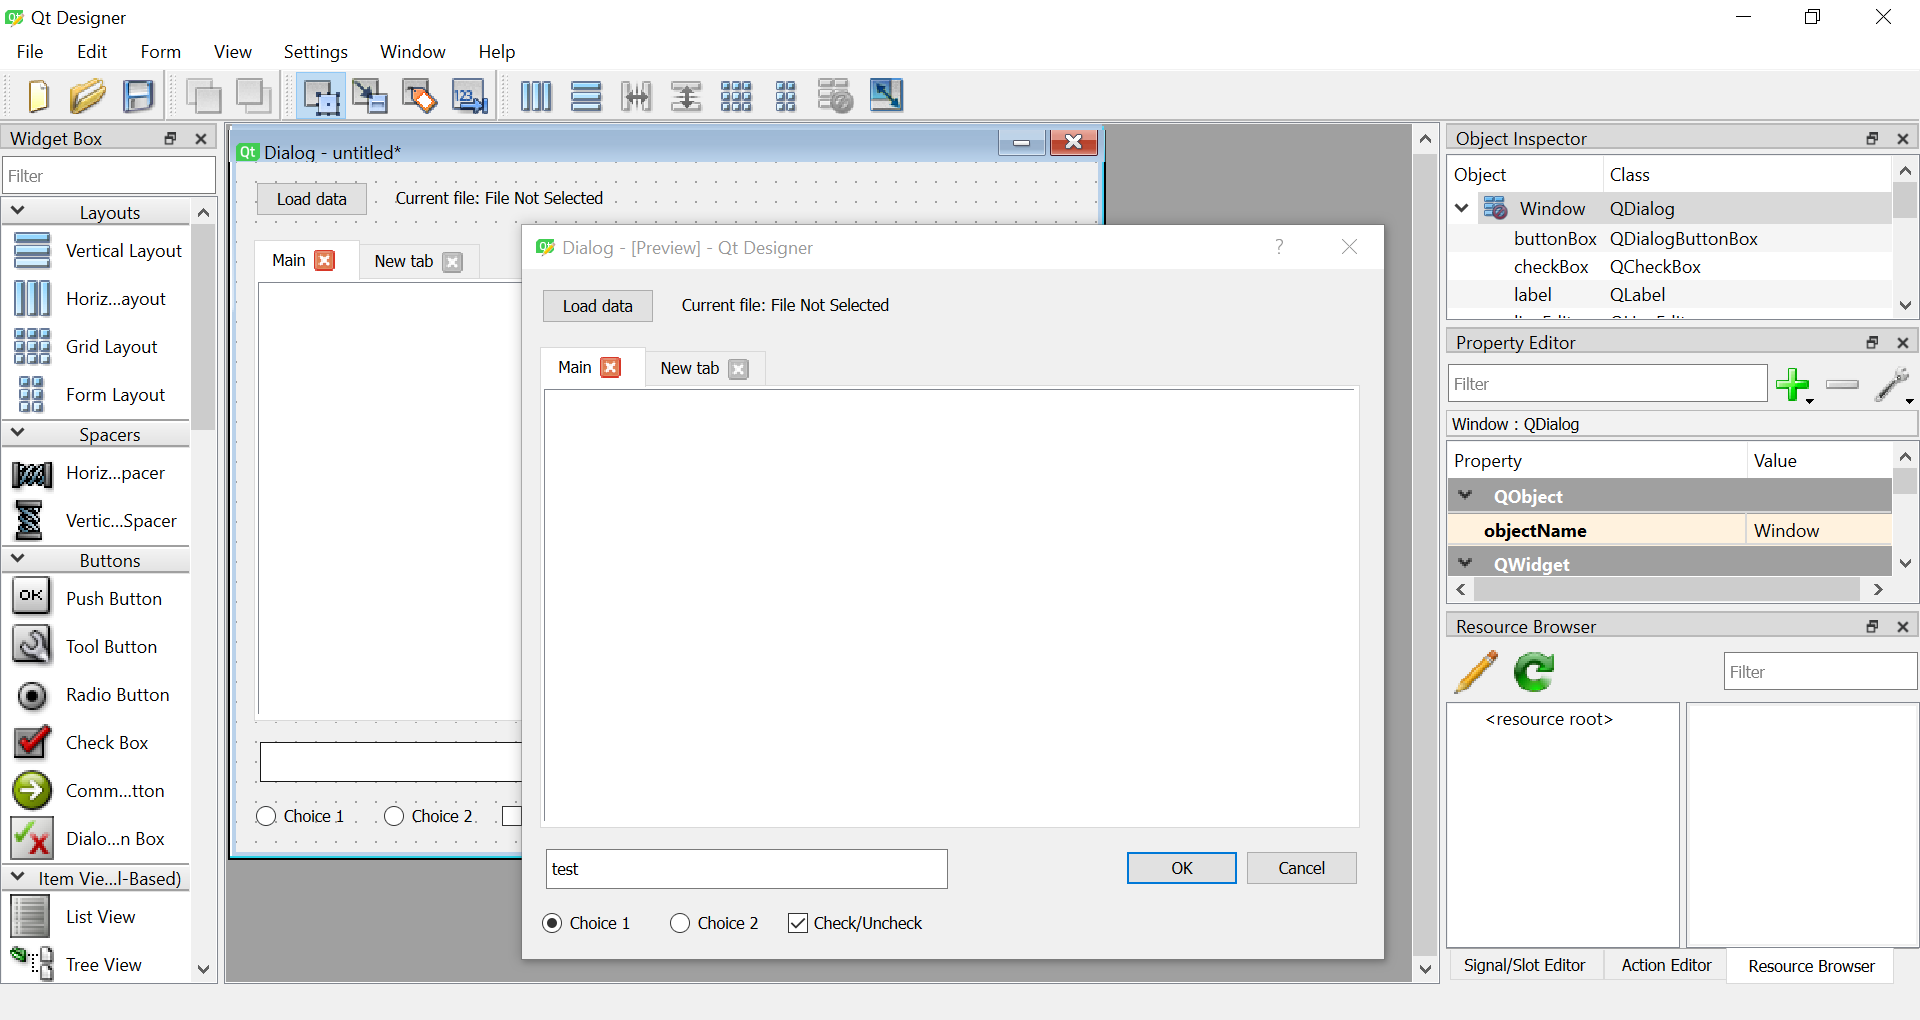
\includegraphics[width=\linewidth,height=9cm]{QtDesigner.png}
    \caption{Ukázka použití nástroje QtDesigner}
    \label{fig:QtDesigner}
\end{figure}
\\
\noindent Z pohledu skriptu je proto elegantnějším řešením napsat GUI ručně. Tento přístup je ale na druhou stranu časově výrazně náročnější. Obecně lze říci, že použití QtDesigneru je výhodné při tvorbě jednoduchých aplikací, zejména pro osobní použití, nebo jako podpůrného nástroje pro začátečníky.
\\
\noindent Pro komplexnější úlohy se tedy lépe hodí ruční psaní GUI. To sice vyžaduje jistou programovací zkušenost, nicméně nabízí oproti QtDesigneru určitou svobodu v možnosti rozšíření nabídky ovládacích prvků nadefinováním vlastních přímo v kódu a zároveň umožňuje docílit větší přehlednosti a úspornosti skriptu použitím pouze nezbytných příkazů.
\\
\\
Nakonec byla pro srovnání obou frameworků v každém z nich generována  jednoduchá demonstrační aplikace, jejíž grafické rozhraní sestává z hlavního okna a dvou tlačítek (viz obr. č. \ref{fig:myfirstgui}). Při stisku tlačítka \texttt{Hello world!} program vypíše na konzoli pozdrav \uv{Hello world!}, při stisku druhého tlačítka se program ukončí. Skript obou variant implementace je dostupný v příloze \ref{PrilohaA} této práce.

\begin{figure}[h!]
\centering
\begin{minipage}[b][4cm]{5cm}
  \centering
  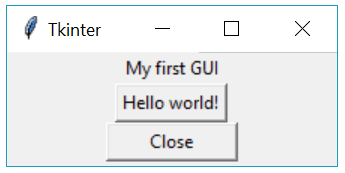
\includegraphics[width=\linewidth]{tkinter_myfirstgui.png}\\
  tkinter
  \captionsetup{labelformat=empty}
\end{minipage}\hspace{1.5cm}
\begin{minipage}[b][4cm]{5cm}
  \centering
  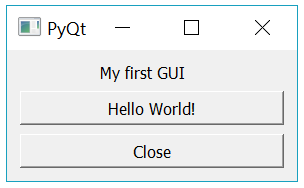
\includegraphics[width=\linewidth]{pyqt_myfirstgui.png}\\
  PyQt
  \captionsetup{labelformat=empty}
\end{minipage}
\caption{Aplikace \texttt{Hello world!} - ukázka výstupů srovnávaných frameworků}
\label{fig:myfirstgui}
\end{figure}

\ldots .


\newpage
\section{Zpracování signálu}
Tato kapitola se zaměřuje na vnitřní podstatu programu pro zpracování krystalografických dat, tj. na číslicové zpracování signálu, od stručného nastínění teorie signálů (viz sekce \ref{sec:signal}), přes problematiku jejich zpracování až ke konkrétním příkladům číslicových filtrů implementovaných v rámci programu (viz sekce \ref{sec:filtr1} až \ref{sec:filtr4}).

\subsection{Signály} \label{sec:signal}
Signály jsou nositeli informace o podstatě svého zdroje, která je reprezentována okamžitou změnou jedné či více fyzikálních veličin v čase. \cite{uhlíř&sovka2002} Podle povahy signálů je lze dělit např. na spojité a diskrétní. Spojité signály jsou definované pro nekonečně mnoho hodnot nezávisle proměnné veličiny, u diskrétních signálů nezávisle proměnná nabývá pouze hodnot celočíselných. Signály mohou být diskrétní i pro hodnoty závisle proměnné (např. v amplitudě), v takovém případě je nazýváme kvantovanými, popř. číslicovými, jsou-li diskrétní jak v čase, tak v amplitudě (viz obr. č. \ref{fig:signal}).
\begin{figure}[h!]
\centering
\begin{minipage}[c]{5cm}
  \centering
  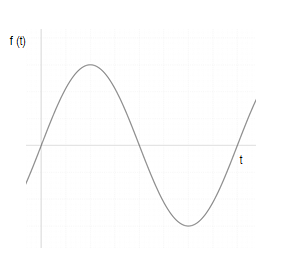
\includegraphics[width=\linewidth]{analogový.png}\\
  a)
  \captionsetup{labelformat=empty}
\end{minipage}\hspace{1cm}
\begin{minipage}[c]{5cm}
  \centering
  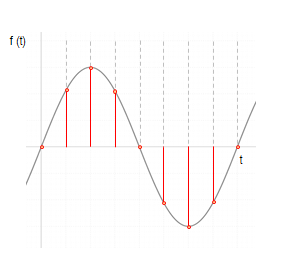
\includegraphics[width=\linewidth]{vzorkovaný.png}\\
  b)
  \captionsetup{labelformat=empty}
\end{minipage}\vspace{0.3cm}
\begin{minipage}[b]{5cm}
  \centering
  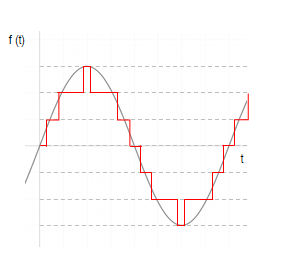
\includegraphics[width=\linewidth]{kvantovaný.png}\\
   c)
   \captionsetup{labelformat=empty}
\end{minipage}\hspace{1cm}
\begin{minipage}[b]{5cm}
  \centering
  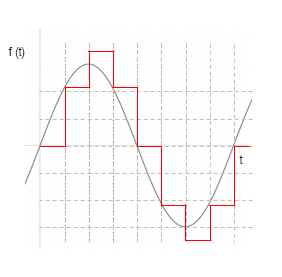
\includegraphics[width=\linewidth]{číslicový.png}\\
  d)
  \captionsetup{labelformat=empty}
  
\end{minipage}
\caption{Druhy signálů: a) analogový, b) vzorkovaný, c) kvantovaný, d) číslicový.}
\label{fig:signal}
\end{figure}
\newline
Dalším kritériem pro klasifikaci signálů je jejich chování v čase. To je dáno okolnostmi jejich vzniku, fyzikální podstatou a dalšími faktory. V případě, že lze předvídat časový průběh signálu, nazýváme jej signálem deterministickým. V opačném případě, tedy pokud má jeho chování zcela náhodnou povahu, jde o signál stochastický.
Běžné signály jsou obvykle analogového charakteru, tj. spojité v čase i amplitudě. Pro možnost jejich dalšího zpracování je proto potřeba je při jejich experimentálním získávání souběžně diskretizovat - sledovaná veličina je snímána pouze v určitých časových okamžicích (vzorkování) a zároveň jsou pomocí vestavěných A/D převodníků kvantovány. Výsledný signál je tak plně digitální, tedy diskrétní v čase i amplitudě. Takto upravený signál je možné podrobit číslicovému zpracování.
To se provádí z důvodu potlačení, příp. zvýraznění určitých složek signálu. Složky, které jsou z pohledu sledovaného děje rušivé se nazývají šum a do signálu se dostávají už ve chvíli jeho vzniku, buď z vnitřního prostředí zdroje nebo vlivem okolí. Mezi základní nástroje signálového zpracování patří
analogová a číslicová filtrace, časová, spektrální nebo časově-frekvenční analýza a další. Vzhledem ke komplexnosti problematiky zpracování signálu se tato práce zaměří pouze na jeden z jejích nástrojů, a to na číslicovou filtraci.

%Zpracování signálu ne vždy poskytuje optimální výsledky, záleží zejména na povaze signálu a také na jeho zašuměnosti, která je dána poměrem signál-šum (SNR, z angl. \textit{signal to noise ratio}).

\subsection{Číslicová filtrace signálu} \label{sec:filtry)}
Filtrace signálu je proces zprostředkovávaný systémem, číslicovým filtrem, při němž dochází ke změně frekvenčního spektra vstupního signálu za účelem zvýraznění, resp. potlačení některých jeho složek. \cite{filtracedef}
Číslicový filtr charakterizují tři základní vlastnosti - impulzní, přenosová a frekvenční charakteristika, které poskytují kompletní představu o chování filtru. Impulzní charakteristika udává chování filtru vyjádřené jeho odezvou na jednotkový puls. Na jejím základě lze filtry rozdělit na ty s konečnou  impulzní odezvou (nebo-li FIR, z angl. \textit{finite impulse response}), jejichž impulzní odezva má konečný počet nenulových hodnot, a na ty s nekonečnou impulzní odezvou (nebo-li IIR, z angl. \textit{infinite impulse response}), u nichž je počet nenulových hodnot impulzní odezvy nekonečný. Hlavní předností FIR filtrů je jejich stabilita a také poměrně snadný matematický popis, na druhou stranu jejich chování je poměrně vzdálené od chování ideálních filtrů (obr. č. \ref{fig:filtryfrekvs}). Pro IIR filtry je naopak typické  \ldots .
\newline
Převedením impulzní charakteristiky do frekvenční oblasti pomocí tzv. Z-transformace je možné získat přenosovou charakteristiku filtru.
\begin{equation}
H (z) = \frac{b_0 + b_1·z^{-1} + ... + b_n·z^{-n}}{1 + a_1·z^{-1} + ... + a_m·z^{-m}}
\end{equation}
Ta udává odezvu filtru na libovolný vstupní signál. Ekvivalentně je možné získat odezvu filtru konvolucí vstupu s jeho impulzní charakteristikou.
\begin{equation}
y [n] = x [n] * h [n] = \sum_{k = -\infty}^{\infty} x[k]·h[n-k]
\end{equation}
Frekvenční charakteristika je odvozena od impulzní charakteristiky pomocí diskrétní Fourierovy transformace (DTFT, z angl. \textit{discrete time Fourier transform}).
\todoin[bordercolor=lavender!80,backgroundcolor=lavender!40]{Pro mě: tady by to chtělo ještě nějak logicky propojit}
\newline\noindent Podle účelu lze pak filtry rozdělit na základě jejich frekvenční selektivity na dolní propusti (angl. \textit{low-pass}), horní propusti (angl. \textit{high-pass}), pásmové propusti (angl. \textit{band-pass}) a pásmové zádrže (angl. \textit{band-stop}). Jak je patrné z obr. č.\ref{fig:filtryfrekvs}, filtry typu propust konzervují požadované frekvence signálu a ostatní potlačují, naopak filtry typu zádrž požadované frekvence potlačí a zbytek signálu ponechají bez zásahu.
\begin{figure}[hbt!]
\centering
\begin{minipage}[b]{6.5cm}
  \centering
  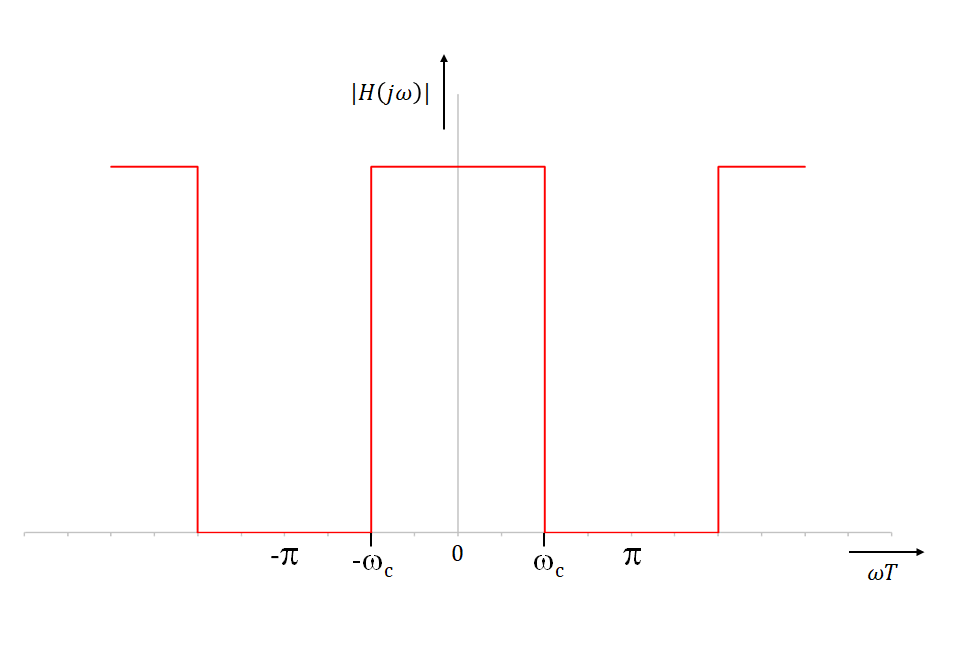
\includegraphics[width=\linewidth]{lowpass.png}\\
  a) dolní propust
  \captionsetup{labelformat=empty}
\end{minipage}\hspace{0.5cm}
\begin{minipage}[b]{6.5cm}
  \centering
  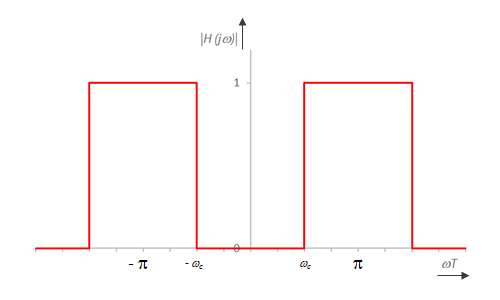
\includegraphics[width=\linewidth]{highpass.png}\\
  b) horní propust
  \captionsetup{labelformat=empty}
\end{minipage}\vspace{0.8cm}
\begin{minipage}[b]{6.5cm}
  \centering
  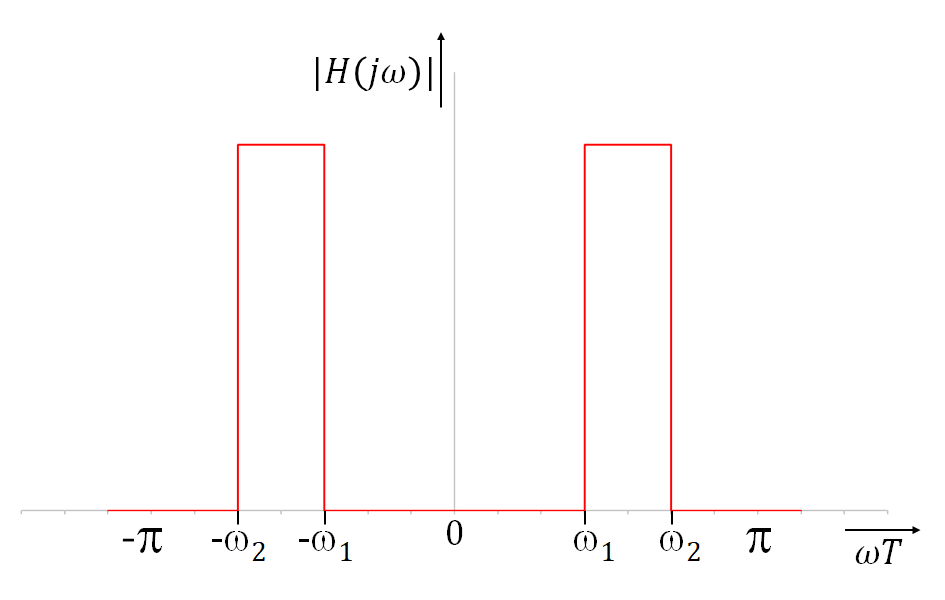
\includegraphics[width=\linewidth]{passband.png}\\
  c) pásmová propust
  \captionsetup{labelformat=empty}
\end{minipage}\hspace{0.5cm}
\begin{minipage}[b]{6.5cm}
  \centering
  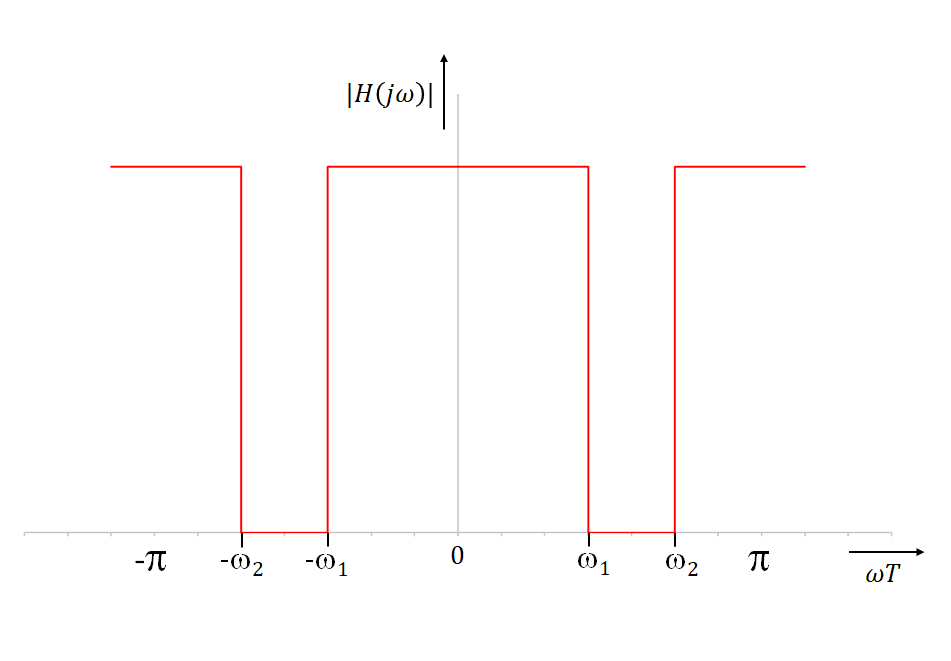
\includegraphics[width=\linewidth]{bandstop.png}\\
  d) pásmová zádrž
  \captionsetup{labelformat=empty}
\end{minipage}
\caption{Frekvenční charakteristiky ideálních číslicových filtrů}
\label{fig:filtryfrekvs}
\end{figure}
% v praxi chování filtrů neideální
% úspěšnost filtrace dána zašuměností signálu (SNR)
\todoin[bordercolor=lavender!80,backgroundcolor=lavender!40]{Pro mě: tady by to chtělo ještě nějak logicky propojit}
\newline\noindent Dále budou blíže popsány konkrétní filtry, které byly zařazeny do programu pro zpracování krystalografických dat.

\newpage

\subsubsection{Filtr s nulovým fázovým posunem}
\label{sec:filtr1}
Prvním z číslicových filtrů využitých v rámci programu je filtr s nulovým fázovým posunem. K implementaci tohoto druhu filtrace jsou využívány jak filtry FIR typu, tak IIR typu. Ty jsou výpočetně méně náročné, zároveň ale vykazují fázové zkreslení způsobené nelinearitou frekvenční charakteristiky filtru, kdy dochází k nestejnému zpožďování různých složek signálu. U FIR filtrů k tomuto jevu také dochází, zkreslení je však vlivem lineární frekvenční charakteristiky konstantní a nedochází proto k deformaci časové řady. Efekt fázového zkreslení lze částečně potlačit právě zero-phase filtrací. \textcolor{lavender}{V rámci programu byl použit filtr lineární (viz \ref{sec:exp_filtrace})}.

Pro docílení nulového fázového posunu se provádí filtrace v dopředném a zpětném směru. To je možné provést dvěma způsoby, buď je nejprve signál filtrován, následně překlopen v čase, poté znova filtrován a nakonec opět překlopen v čase nebo jsou tyto operace provedeny v opačném pořadí, tj. nejprve překlopení signálu v čase a poté filtrace. Oba tyto postupy poskytují ekvivalentní výsledky, jedná se tedy pouze o formální odlišnost ve vnitřním fungování zero-phase systému. Schéma filtrace s nulovým fázovým posunem je znázorněno na obr. č. \ref{fig:zerophase}.
\begin{figure}[hbt!]
  \centering
  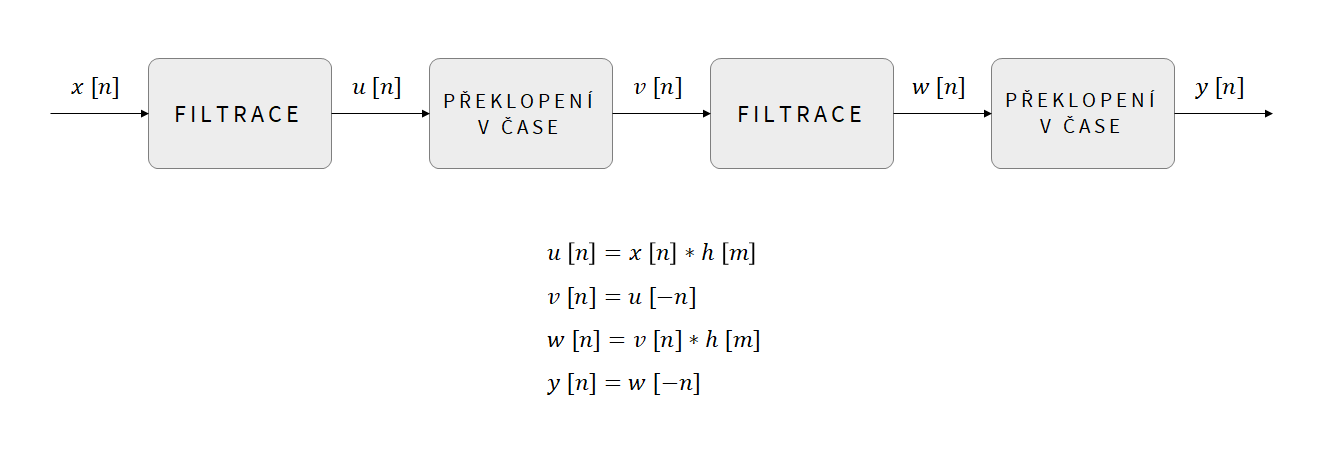
\includegraphics[width=\linewidth]{zero-phase_moje.png}
  \caption{Princip filtrace s nulovým fázovým posunem}
  \label{fig:zerophase}
\end{figure}

\subsubsection{Savitzky-Golay filtr}
\label{sec:filtr2}
polynomiální filtr
\ldots .

\subsubsection{Mediánový filtr}
\label{sec:filtr3}
nahrazuje \(x^{stare^{´}}\) mediánem hodnot v okně
\ldots .

\subsubsection{Exponenciální vyhlazování}
\label{sec:filtr4}
\(y_0 = x_0\)\\
\(y_i = x_i · \alpha + y_{i-1} · (1-\alpha)\)\\
\ldots .

%%

% praktická část
\newpage
\section{Tvorba uživatelského rozhraní a zpracování krystalografických dat}

\subsection{Hlavní okno a funkce}
\ref{PrilohaA}.
\subsubsection{Import dat a jejich vizualizace}
\cite{petz08}.
\subsubsection{Práce s daty, výběr kanálu}
\ldots .
\subsubsection{Záložky a funkce}
\ldots .

\subsection{Filtrace signálu}\label{sec:exp_filtrace}

\subsection{Export dat}
\ldots .

\newpage
\section{Výsledky a diskuse}

\newpage
\section{Závěr}


% seznam literatury
\newpage
\addcontentsline{toc}{section}{Literatura}

\bibliography{citace}
\bibliographystyle{ieeetr}
%%

% přílohy
\newpage

\appendix
%
\section{Zdrojové kódy miniaplikace \texttt{Hello world!}}
\label{PrilohaA}
\subsection{Miniaplikace \texttt{Hello world!} vytvořená v tkinter}
\lstinputlisting[language=python]{tkinter_hello.py}

\subsection{Miniaplikace \texttt{Hello world!} vytvořená v \texttt{PyQt5}}
\lstinputlisting[language=python]{pyqt_hello.py}
%
\section{Zdrojový kód programu pro zpracování krystalografických dat}
\label{PrilohaB}
\lstinputlisting[language=python]{crystallography_data_processing_zemlovak.py}

\end{document}
